%%%%%%%%%%%%%%%%%%%%%%%%%%%%%%%%%%%%%%%%%%%%%%%%%%%%%%%%%%%%%%%%%%%%%%%%%%%%%%%%%%%%%%
% TEMPLATE FOR Praktikum P3B
% This template uses the Memoir class. It is a very powerful class for creating documents such
% as reports, papers and theses. You can find more information at CTAN, the Comprehensive
% TeX Archive Network. These is a long manual that describes how to use Memoir.
% https://www.ctan.org/pkg/memoir?lang=en
% Sven Buschke
% Last Update: 2021-08-18
%%%%%%%%%%%%%%%%%%%%%%%%%%%%%%%%%%%%%%%%%%%%%%%%%%%%%%%%%%%%%%%%%%%%%%%%%%%%%%%%%%%%%

%------------------------------------------------------------------------------------
%	EDIT THIS BLOCK
%------------------------------------------------------------------------------------
\newcommand{\studentfullname}{Sven Buschke}			% change to your name
\newcommand{\matrikelnumber}{27205317}				% enter your student number 
\newcommand{\dateexperiment}{26. August 2021}				% change to your partner's name
\newcommand{\timeexperiment}{13:30-18:00 Uhr}				% enter your partner's student number
\title{P3B-Versuch 1/2 ROE --- Röntgenstrahlung: Bragg-Reflexion und Röntgenfluoreszenzanalyse}					% change to the title of the experiment
\author{\studenfullname}				% you don't have to change this
\date{25.\ August 2021}										% this fills in today's date - don't change



%------------------------------------------------------------------------------------
%	FORMATTING STUFF
%------------------------------------------------------------------------------------

\documentclass[12pt,oneside,oldfontcommands]{memoir}


%-----------------------------------------------------------------------------------
%	MARGIN AND HEADER/FOOTER SIZES
%------------------------------------------------------------------------------------
\setlrmarginsandblock{2.5cm}{2.5cm}{*}  		% left/right margins
\setulmarginsandblock{2.5cm}{2.5cm}{*} 			% top/bottom margins
\checkandfixthelayout							% checks the layout is correct
\setlength{\parindent}{0in}  					% no indent on start of paragraph
							

%-------------------------------------------------------------------------------------
%  PACKAGES
%-------------------------------------------------------------------------------------
\usepackage{amsmath,amsthm,amssymb,amsfonts}			% math fonts
\usepackage[german]{babel}								% hyphenation rules for German
\usepackage{graphicx}									% for importing pdf files 
\usepackage{siunitx}									% si units - extremely useful
\usepackage[usenames,dvipsnames,svgnames,table]{xcolor}	% defines the dvips color names
\usepackage{color,soul} 								% for highlight hi - hyphenation, underlining
%\usepackage{libertine}
%\usepackage{libertinust1math}
%\usepackage[T1]{fontenc}
\usepackage{fontspec}
\usepackage{pdfpages}
\setmainfont{Linux Libertine O}%
   [Ligatures={Common,Historic}, Numbers=OldStyle]
\setulcolor{red} 										% set underline color
\setstcolor{green} 										% set overstriking color
\sethlcolor{green} 										% set highlighting color


%--------------------------------------------------------------------------------------------
%  GRAPHICS PATH
%--------------------------------------------------------------------------------------------
\graphicspath{{figures/}}								% put your figures in a folder called figures



%---------------------------------------------------------------------------
%  SOME NEW FUNCTIONS FOR IMPORTING FIGURES
%---------------------------------------------------------------------------
\newcommand{\placefigure}[1]{\centerline{\includegraphics[width=2 in]{#1}}} 
\newcommand{\placefigureandscale}[2]{\centerline{\includegraphics[width=#2 in]{#1}}} 



%-------------------------------------------------------------------------------------
%	TITLE PAGE MACRO
%------------------------------------------------------------------------------------
\makeatletter
\def\maketitle{%
  \null
  \thispagestyle{empty}
  \begin{center}\leavevmode
       \normalfont 
       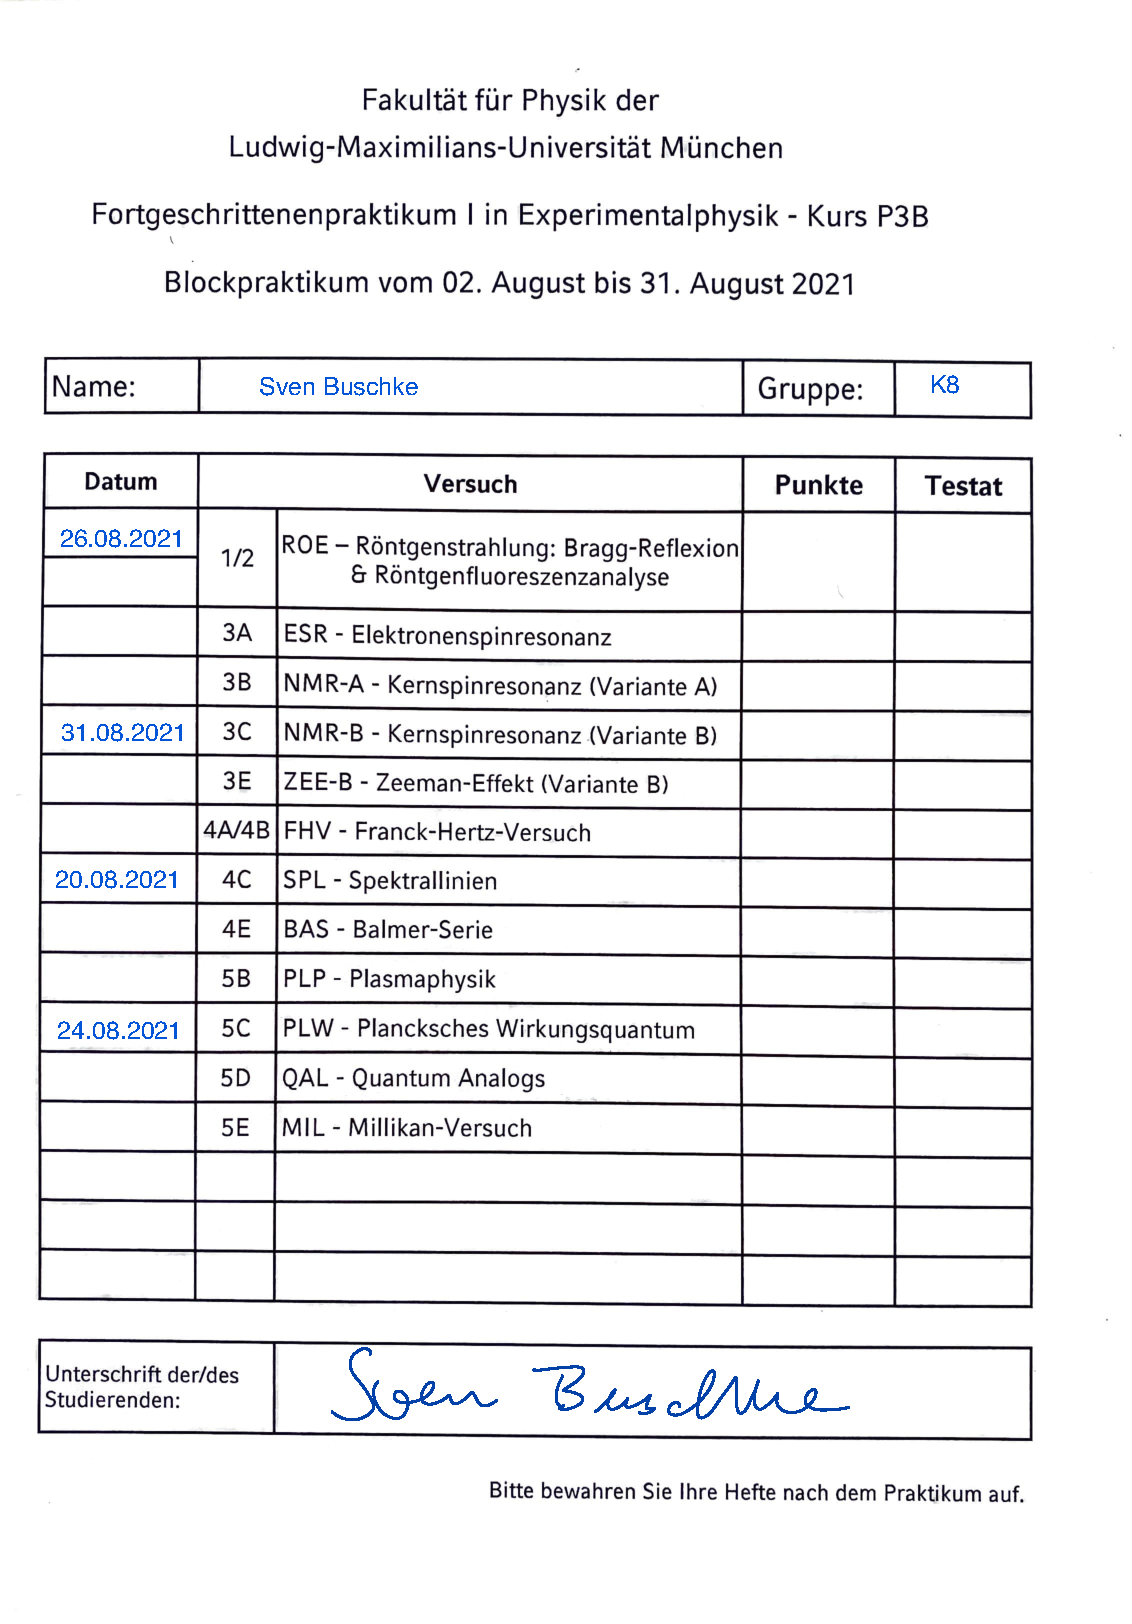
\includepdf[pages=1,scale=0.9,pagecommand={}]{Deckblatt-P3B-signed-20210825.pdf}
       %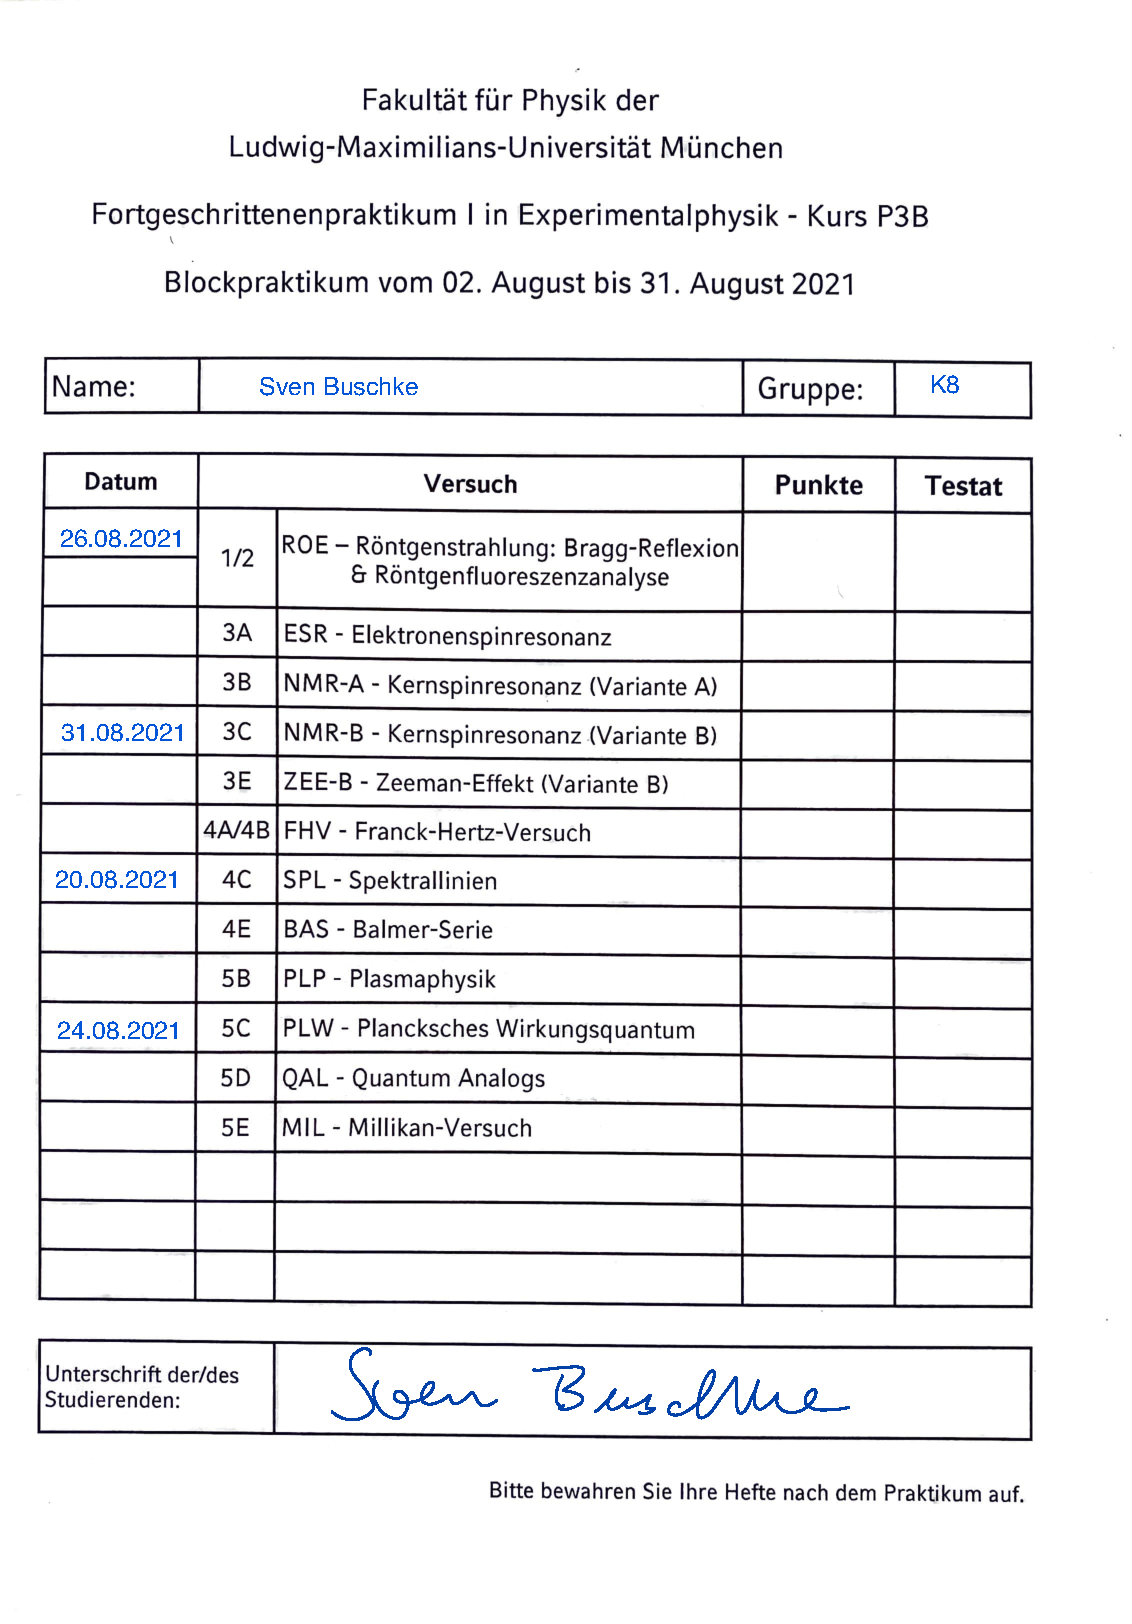
\includegraphics[width=.96\columnwidth]{Deckblatt-P3B-signed-20210825.pdf}
       \newpage
       
\includegraphics[width=0.165\columnwidth]{lmu-seal.pdf}
       
\includegraphics[width=0.35\columnwidth]{lmu-logo.pdf}
       \vskip 0.5cm   
       \textsc{\Large P3B-Praktikum}\\[0.5 cm]
	     {\large \@date\par}
       \vskip 1.0cm
	\rule{\linewidth}{0.2 mm} \\[0.4 cm]
	{ \huge \bfseries \@title}\\
	\rule{\linewidth}{0.2 mm} \\[1.5 cm]
	
	\begin{minipage}{0.5\textwidth}
		\begin{flushleft} \large
			\emph{Name:} \studentfullname\\
			Matrikelnummer: \matrikelnumber
			\end{flushleft}
			\end{minipage}
			\begin{minipage}{0.4\textwidth}
			\begin{flushleft} \large
			Versuchstermin: \dateexperiment\\
			Versuchsdauer: \timeexperiment
		\end{flushleft}
	\end{minipage}\\[2 cm]
   \end{center}
   \vfill
   \null
   \cleardoublepage
  }
\makeatother



%-------------------------------------------------------------------------------------------
%	START OF DOCUMENT
%--------------------------------------------------------------------------------------------

\begin{document}
%\large 
\maketitle
\frontmatter
\let\cleardoublepage\clearpage
\mainmatter
\sloppy



%--------------------------------------------------------------------------------------------
%	RESULTS AND ANALYSIS
%--------------------------------------------------------------------------------------------

\setcounter{tocdepth}{3}
\tableofcontents

\section{Vorbereitung Versuch 1/2 ROE --- Röntgenstrahlung: Bragg-Reflexion und Röntgenfluorenszenzanalyse}
\subsection{Physikalische Grundlagen}
Mit den wellenlängenabhängigen Beugungswinkeln soll in diesem Versuch im Rahmen der Bragg-Reflexion gemäß Versuchsanleitung das Spektrum einer Molybdän-Anode untersucht werden. Der Versuch besteht aus fünf Teilversuchen.
\subsubsection{Stichworte}
\paragraph{Röntgenröhre}
Eine Röntgenröhre besteht im Wesentlichen aus der Kathode und der Anode. Die Kathode emittiert Elektronen. In Richtung der Anode werden die Elektronen stark beschleunigt, bis zum Auftreffen. Hier erfolgt eine Abbremsung. Im Zuge der Abbremsung kommt unter anderem zu Röntgenstrahlung (charakteristische Röntgenstrahlung) und zur Bremsstrahlung.
Letzgenannte verläuft kontinuierlich. Die charakteristische Strahlung hängt vom Material ab.

\paragraph{Linienspektrum eines Stoffes, Schalenmodell, mögliche Übergänge (Quantenmechanik)}
Die Elektronen sind auf Schalen angeordnet, konfiguriert gemäß Notation der Quantenphysik in n, l, $m?l$, s, $m_s$. Hier kommt es zu Übergängen innerhalb der Energieniveaus. Durch den Übergang kommt es zu Abstrahlungen, d.h. Photonen kommen ins Spiel. Hier ist die Formel $E = h\frac{c}{\lambda}$, mit der charakteristischen Wellenlänge für den jeweiligen Übergang, die auch das Linienspektrum des Atoms festlegt.

\paragraph{Röntgenstrahlung, Bremsstrahlung, charakteristische Strahlung}
Durch die Ionisation eines Atoms bzw. durch das Bringen in eine freue Schale, die ein Elektron, durch ein anderes angeregt, aus einer niedrigen Schale in der Anode ausbringt. Hierdurch kommt es zur charakteristischen Strahlung. Die Übergänge finden sich wieder in den K-alpha-beta-Linien.

\paragraph{Zustandekommen der charakteristischen Strahlung im Röntgenspektrum}
Siehe von vorhin

\paragraph{Bragg-Reflexion}
Strahlen werden von einem Kristallgitter reflektiert oder transmittiert. Hier kann es zu Interferenz der Strahlen im Zuge der Reflektion kommen. Je nach Winkel interferieren verschiedene Ebenen im Kristall. Hieraus lässt sich auf die Kristallgitterstruktur schließen. Es gilt $2d \sin (\theta) = m \lambda$, mit dem Bragg-Winkel $\theta$.

\paragraph{Duane-Huntsches-Verschiebungsgesetz, Erklärung der Abhängigkeit zwischen Grenzwellenlänge und Röhren-Hochspannung mit einfachen quantenmechanischen Überlegungen}
Ein Elektron hat die kinetische Eneergie als maximale Energie, bestimmt durch die Beschleunigungsspannung. Es gilt $eU = h \frac{c}{\lambda}$, woraus sich $lambda$ bestimmen lässt: $\lambda = \frac{hc}{eU}$

\paragraph{Moseleysches Gesetz (Herkunft, Grundannahmen, ...)}
Mit dem Moseleyschen Gesetz wird der Zusammenhang zwischen Element-Wellenlänge und Kernladungszahl hergestellt. Es gilt: $E = 1/2 m c^2 a^(Z-1)^2 \frac{1}{1^2}- \frac{1}{2^2}$ oder auch $\sqrt{\frac{\nu}{cR_{\infty}}} = (Z-1)\sqrt{1-1/4}$
 
\paragraph{Spektrallinien (Absorptions- und Emissionsspektrum}
Das Emissionsspektrum ist das Spektrum, das entsteht, wenn ein Photon von einem Elektron von einem höheren auf ein niedrigeres Niveau geht. Das Absorptionsspektrum ist der andere Fall, eben, wenn ein Photos absorbiert wird und ein Elektron auf ein höheres Niveau bringt.

\paragraph{Fluoreszenz / sekundäre Anregung}
Die Emission von Licht, das durch Materialanregung mit Licht entseht, ist die Fluoreszenz.

\paragraph{Detektion von Röntgenstrahung: Geiger-Müller-Zählrohr und Halbleiterdetektor}
Beim Geiger-Müller-Zählrohr liegt eine Spannng an zwischen einer Kathode, häufig in Zylinderform und einem Draht. Hierbei kommt es beim Vorliegen von Röntgenstrahlung zu Ionisierung von Atomen im umgebenen Gas. Hierbei entsteht ein Strom, der gemessen werden kann. Bei der Diode gibt es nur eine Richtung, bei dem Strom fließen kann, in der anderen, der Sperrrichtung, fließt kein Strom.

\subsubsection{Theoretischer Hintergrund / Überblick Versuche}
\paragraph{Teilversuch 1: Bragg-Reflexion}
\paragraph{Teilversuch 2: Energiespektrum Röntgenröhre}
\paragraph{Teilversuch 3: Duane-Huntsches Verschiebungsgesetz}
\paragraph{Teilversuch 4: Röntgenfluoreszenzanalyse}
\paragraph{Teilversuch 5: Identifikation einer unbekannten Probe}

\section{Versuchsdurchführung und Auswertung}
\subsection{Teilversuch 1: Bragg-Reflexion}
\subsubsection{Versuchsvorbereitung, Grundlagen des Versuches, Erläuterung verwendeter Formelzeichen, Versuchsziel, Erläuterung der Messmethoden, schematische Skizzen, Planung der Durchführung, Versuchsplanung, Versuchsdurchführung}

Hier wird die charakteristische Röntgenstrahlung gemessen, des Molybdän.

\subsubsection{Versuchsergebnisse und -auswertung}
Versuchsergebnisse und Auswertung.

\subsection{Teilversuch 2: Energiespektrum Röntgenröhre}
\subsubsection{Versuchsvorbereitung, Grundlagen des Versuches, Erläuterung verwendeter Formelzeichen, Versuchsziel, Erläuterung der Messmethoden, schematische Skizzen, Planung der Durchführung, Versuchsplanung, Versuchsdurchführung}
Hier werden verschiedene Energiespektren einer Röntgenröhre gemessen in Abhängigkeit der Beschleunigungsspannung.

\subsubsection{Versuchsergebnisse und -auswertung}
Versuchsergebnisse und Auswertung.

\subsection{Teilversuch 3: Duane-Huntsches Verschiebungsgesetz}
\subsubsection{Versuchsvorbereitung, Grundlagen des Versuches, Erläuterung verwendeter Formelzeichen, Versuchsziel, Erläuterung der Messmethoden, schematische Skizzen, Planung der Durchführung, Versuchsplanung, Versuchsdurchführung}
Die Minimalwellenlänge in Abhängigkeit der Beschleunigungsspannung werden hier gemessen, zum Nachweis des Duane-Huntschen Verschiebungsgesetz und zur Bestimmung des Planckschen Wirkungsquantums.

\subsubsection{Versuchsergebnisse und -auswertung}
Versuchsergebnisse und Auswertung.

\subsection{Teilversuch 4: Röntgenfluoreszenzanalyse}
\subsubsection{Versuchsvorbereitung, Grundlagen des Versuches, Erläuterung verwendeter Formelzeichen, Versuchsziel, Erläuterung der Messmethoden, schematische Skizzen, Planung der Durchführung, Versuchsplanung, Versuchsdurchführung}
Hier wird mit Hilfe des Röntgengerätes die Röntgenfluoreszenzanalyse durchgeführt. Hierbei werden ein Kollimator, ein Target und ein Detektor (Goniometer) verwendet. Hierbei wird das Programm Cassy-Lab 2 verwendet.
\subsubsection{Versuchsergebnisse und -auswertung}
Versuchsergebnisse und Auswertung.

\subsection{Teilversuch 5: Identifikation einer unbekannten Probe}
\subsubsection{Versuchsvorbereitung, Grundlagen des Versuches, Erläuterung verwendeter Formelzeichen, Versuchsziel, Erläuterung der Messmethoden, schematische Skizzen, Planung der Durchführung, Versuchsplanung, Versuchsdurchführung}
Hier wird eine unbekannte Probe verwendet wie ein Geldstück, analog zu den obigen Teilversuchen.

\subsubsection{Versuchsergebnisse und -auswertung}
Versuchsergebnisse und Auswertung.


\section{Anhang - Laborheft}
\includepdf[pages=-,scale=0.9,pagecommand={}]{P3B-ROE.pdf}
hier kommt das Laborheft

\end{document}